% \documentclass[compress,12pt]{beamer}
\documentclass[slidestop,compress,12pt]{beamer}
%下面是设置主题的
% \usetheme{Warsaw}
\usetheme{AnnArbor} 
% \usetheme{CambridgeUS}
% \usetheme{JuanLesPins}
% \usecolortheme{whale}
% \usecolortheme{dove}
\usecolortheme{crane}
%设置item前面的小箭头的样式的
%\useinnertheme{default}
\useinnertheme{circles}
\usepackage{color}  %颜色
\usepackage{amsmath,amssymb,latexsym}  %数学
\usepackage{wasysym}
\usepackage{mathrsfs}
\usepackage{graphicx}
\usepackage{caption}
\usepackage{amsmath,amssymb}
\usepackage[export]{adjustbox}

\newcommand{\citepaper}[1]{\color{black}{\scriptsize{$\sun$~\it{#1}}}}
% \usepackage{beamerthemesplit} // Activate for custom appearance

\DeclareMathOperator{\diff}{d\!}
\DeclareMathOperator{\Diff}{D\!}
\newcommand{\im}{\mathrm{i}}
\newcommand{\ee}{\mathrm{e}}

\setbeamertemplate{caption}{\raggedright\insertcaption\par}

\title{Electron Tomography and Its Limitations}
\author{Xin Chen}
\date{\today}

\begin{document}
\def\mean#1{\left< #1 \right>}
\frame{\titlepage}

\section[Achievements]{}

\begin{frame}
    \begin{figure}
        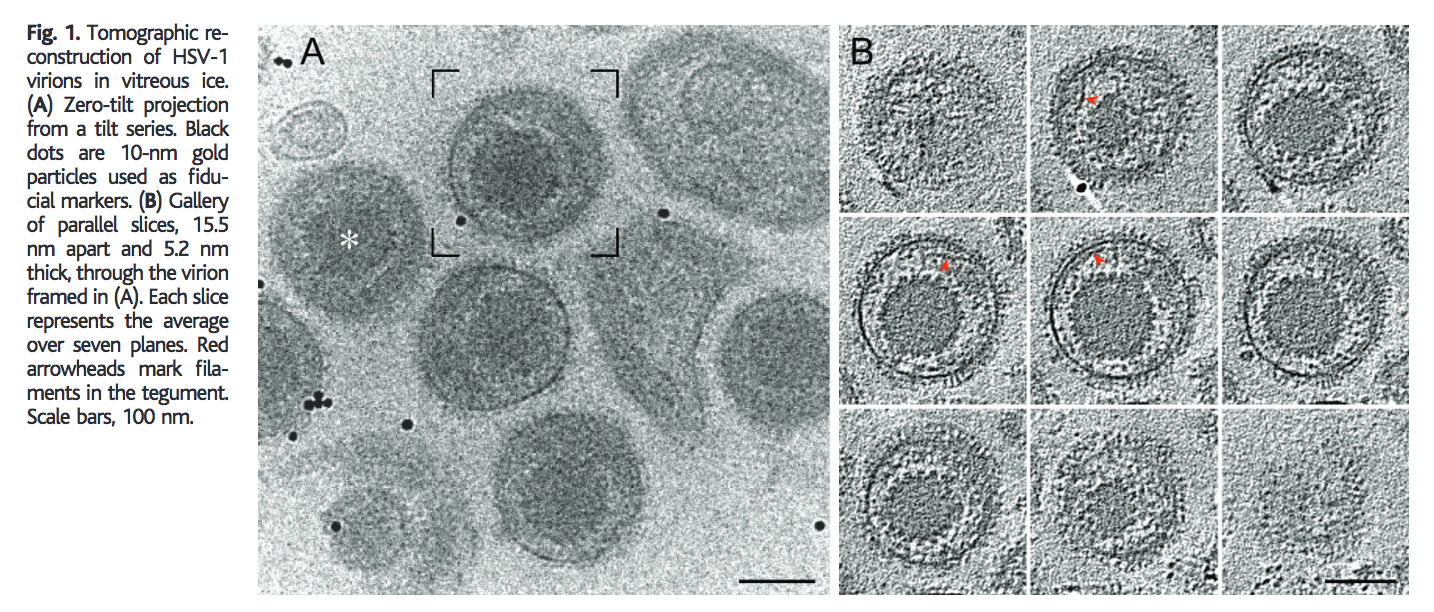
\includegraphics[width=12cm]{imgs/eg1.png}
        \caption{Grünewald, Kay, et al, 2003, resolution: 7nm}
    \end{figure}
\end{frame}

\begin{frame}
    \begin{figure}
        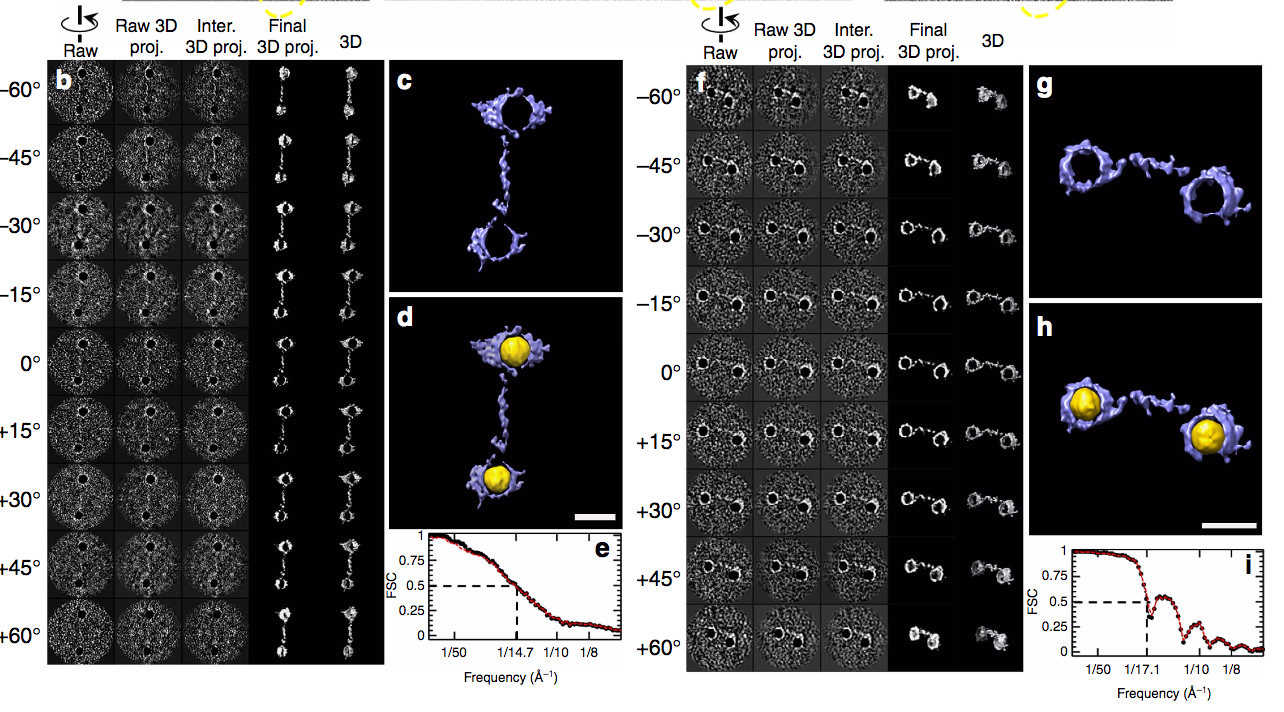
\includegraphics[width=11cm]{imgs/eg2.png}
        \caption{Lei Zhang, et al, 2016, resolution: 17.1\AA, dsDNA:  30nm, gold particle: 6nm}
    \end{figure}
\end{frame}

\section[Radon Transform]{}
\begin{frame}
    \begin{minipage}[c]{0.4\textwidth}
        \begin{figure}
        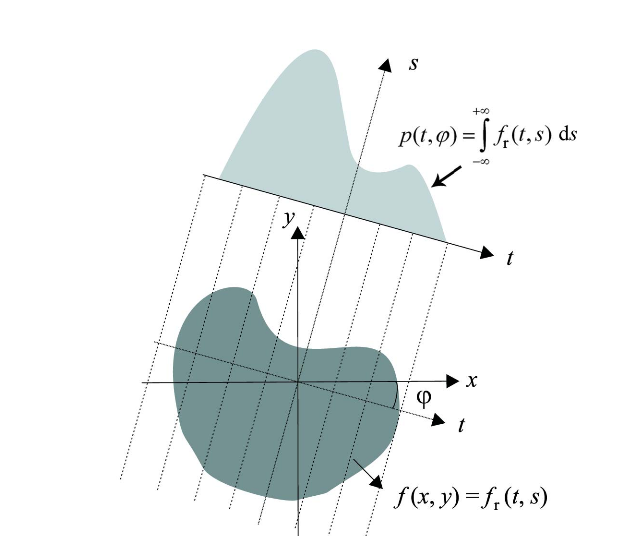
\includegraphics[scale=0.4, left]{imgs/radon1.png}
        \end{figure}
    \end{minipage}%%%
    \begin{minipage}{0.5\textwidth}
    \scriptsize
        \begin{equation}
            \begin{split}
                p(t, \varphi) &= \int\int f(x,y) \delta (x \cos{\varphi} + y \sin{\varphi} - t) \diff x \diff y \notag \\
                P(k, \varphi) &= \text{FT}1[p] = \int\int f(x,y) \ee ^ {-\im k x\cos{\varphi}  - \im k y\sin{\varphi} } \diff x \diff y \\
                & = \int\int f(x,y) \ee ^ {-\im ux  - \im vk} \diff x \diff y \\
                u &= k\cos{\varphi} \\
                v &= k\sin{\varphi}
            \end{split}
        \end{equation}
    \end{minipage}%

    Fourier Slice Theorem: 1D FT of $p(t,\varphi)$ is equal to the slice of 2D FT of $f(x,y)$ at the angle $\phi$ --- the math for iRadon.
    \vspace{-0.23cm}
    \begin{figure}
        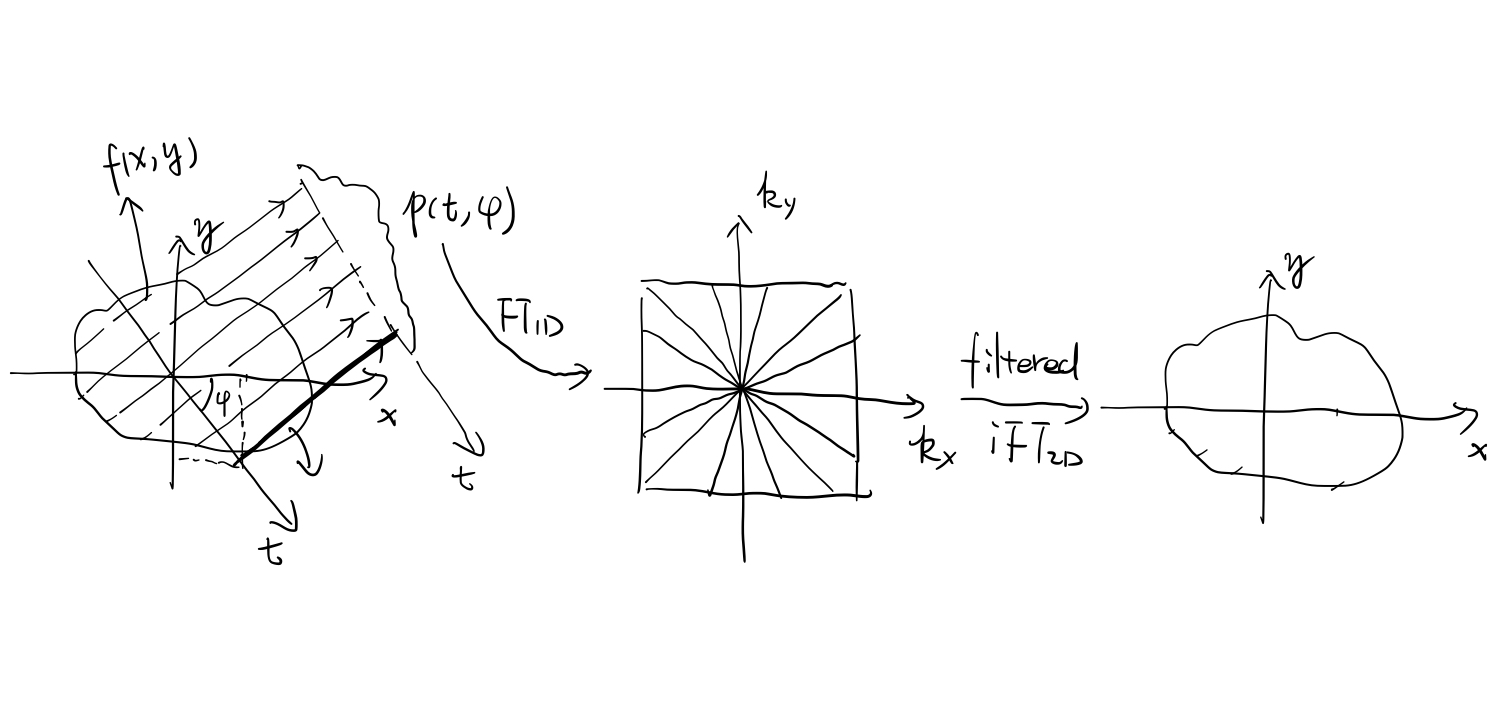
\includegraphics[scale=0.15]{imgs/iradon.jpg}
    \end{figure}

\end{frame}

\begin{frame}
    \begin{figure}
        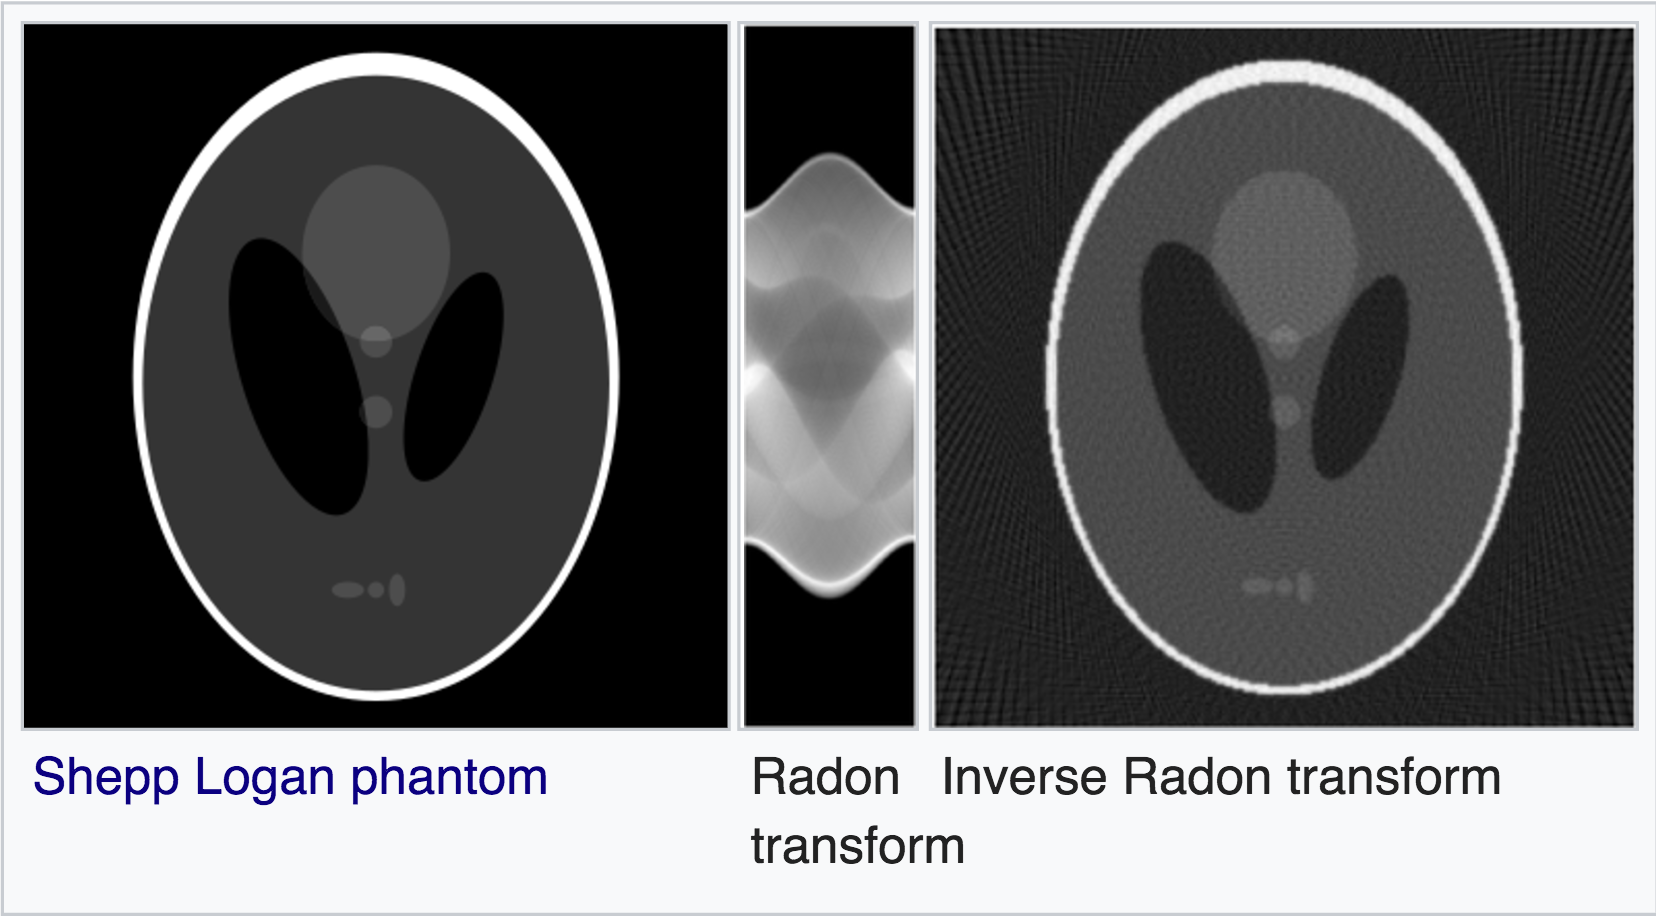
\includegraphics[scale=0.35]{imgs/eg3.png}
    \end{figure}
\end{frame}

\section[3D reconstruction]{}
\begin{frame}
    \begin{figure}
    \centering
        \begin{minipage}{0.2\textwidth}
            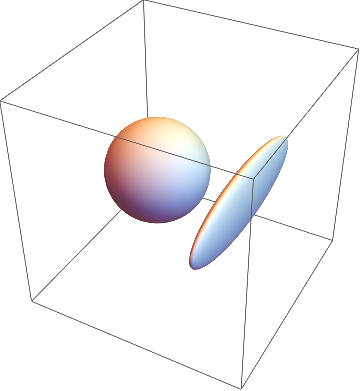
\includegraphics[width=1\linewidth]{imgs/obj.png}
        \end{minipage}%
        \begin{minipage}{0.8\textwidth}
            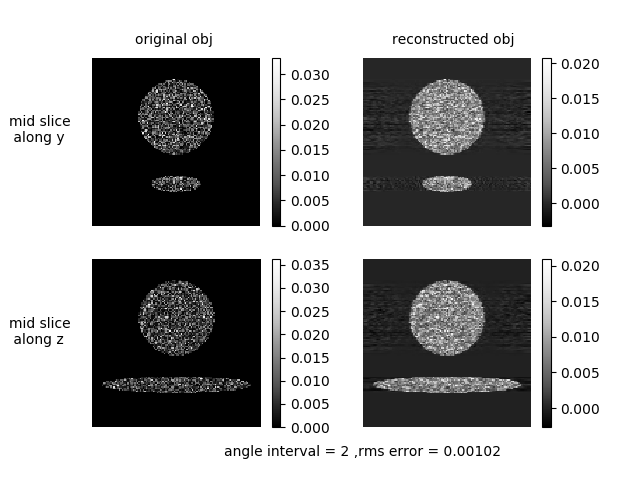
\includegraphics[width=1\linewidth]{imgs/mid_slices.png}
        \end{minipage}
    \end{figure}
\end{frame}

\begin{frame}
    \begin{figure}
        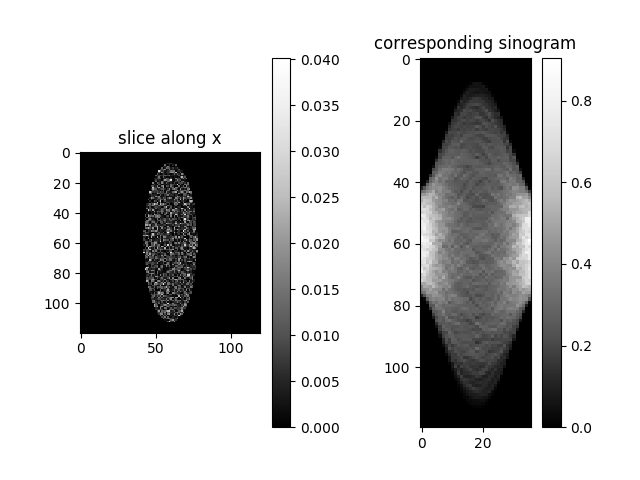
\includegraphics[scale=0.5,left]{imgs/sinogram.png}
    \end{figure}\pause
    \vspace{-3cm}
    \begin{figure}
        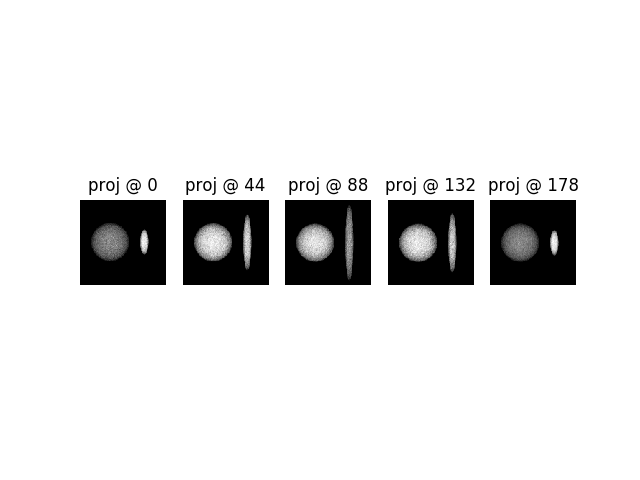
\includegraphics[scale=0.5,right]{imgs/projections.png}
    \end{figure}
\end{frame}
\end{document}























